% !TEX root = 00_MAIN.tex

\chapter{Using Trilinos and Tpetra} \label{sec:trilinos}

The Trilinos~\cite{HB+05} framework is designed to provide linear, nonlinear, and eigen
solvers, as well as discretization and load balancing tools, to parallel
applications.  The tools are designed to run on distributed memory
parallel with multicore or GPU nodes.  
These components can be combined with physics descriptions to 
rapidly construct applications with minimal computer science effort needed
by application developers.

Tpetra~\cite{BH12} is the key linear algebra package in Trilinos.  
Tpetra contains classes
for vectors, multivectors and matrices, with operations performed in CPUs or
GPUs.  Tpetra exploits the Kokkos performance portability layer to enable
computation across a variety of platforms.  GentenMPI uses Tpetra to provide
factor matrices and parallel distribution maps in tensor decomposition.

\section{Parallel distribution and Tpetra Maps} \label{sec:maps}

Tpetra uses the {\tt Map} class to describe the distribution of vectors and
matrices to processors.  Each entity (vector entry, matrix row, matrix column,
etc.) has a unique global identifier (ID).  The {\tt Map} class describes 
the assignment of these IDs to processors.  It also assigns a local identifier
to each global ID on a processor; this local identifier can be used as an 
array index in local vector data.

The default distribution of IDs in a {\tt Map} among processors is 
a linear partition of the IDs; for IDs \{$1,2,\ldots, J$\} on $P$ 
processors, the default {\tt Map} would assign IDs \{$1,2,\ldots,J/P$\} to 
processor 0, IDs \{$J/P+1,\ldots,2J/P$\} to processor 1, and so on.  Users can
obtain other distributions, however, by specifying the number of IDs
to give to each processor or by providing a list of specific IDs to assign
to each processor.

A Tpetra sparse matrix (e.g., {\tt Tpetra::CrsMatrix}) 
has four maps:  a row map, a column map, a domain map, and a range map.  
The row map
of a matrix contains the global indices of each row for which the processor
stores at least one nonzero.  The column map contains the global indices of
each column for which the processor stores at least one nonzero.  Neither
row maps nor column maps need to be ``one-to-one''; that is, many processor
may store a given global ID in their row maps.  The domain and range maps
describe the distribution of the input vectors and output vectors, respectively,
to be used in sparse matrix-vector multiplication.  These maps are 
``one-to-one''; each entry is stored in only one processor's {\tt Map}.

Figure~\ref{fig:trilinosmap} shows examples of the maps associated with a 
matrix $A$, input vector $x$ and output vector $y$.  In the left example, 
$A$ is distributed in a 
row-wise manner, so that all nonzero entries (marked with $x$) in a row
are assigned to a single processor.  The blue processor has nonzeros in
rows 4 and 5; thus, entries 4 and 5 are in its row map.  The nearly dense
row 5 causes the blue processor's column map to have nearly all column 
indices.  The distributions of $x$ and $y$ to processors are identical;
thus, the range and domain maps are identical.   The right example the same
distributions of the input and output vectors, but uses a 
nonzero-based distribution of the tensor.  The blue
processor has nonzero entries in rows 4, 5, and 8; thus, these entries are 
in its row map.  Note that rows 4 and 5 are also in the red processor's
row map.  The column map for the blue processor is smaller in the right 
figure, as the blue processor has nonzeros only in rows 4, 5, 6, and 7.

\begin{figure}[ht]
   \centering
   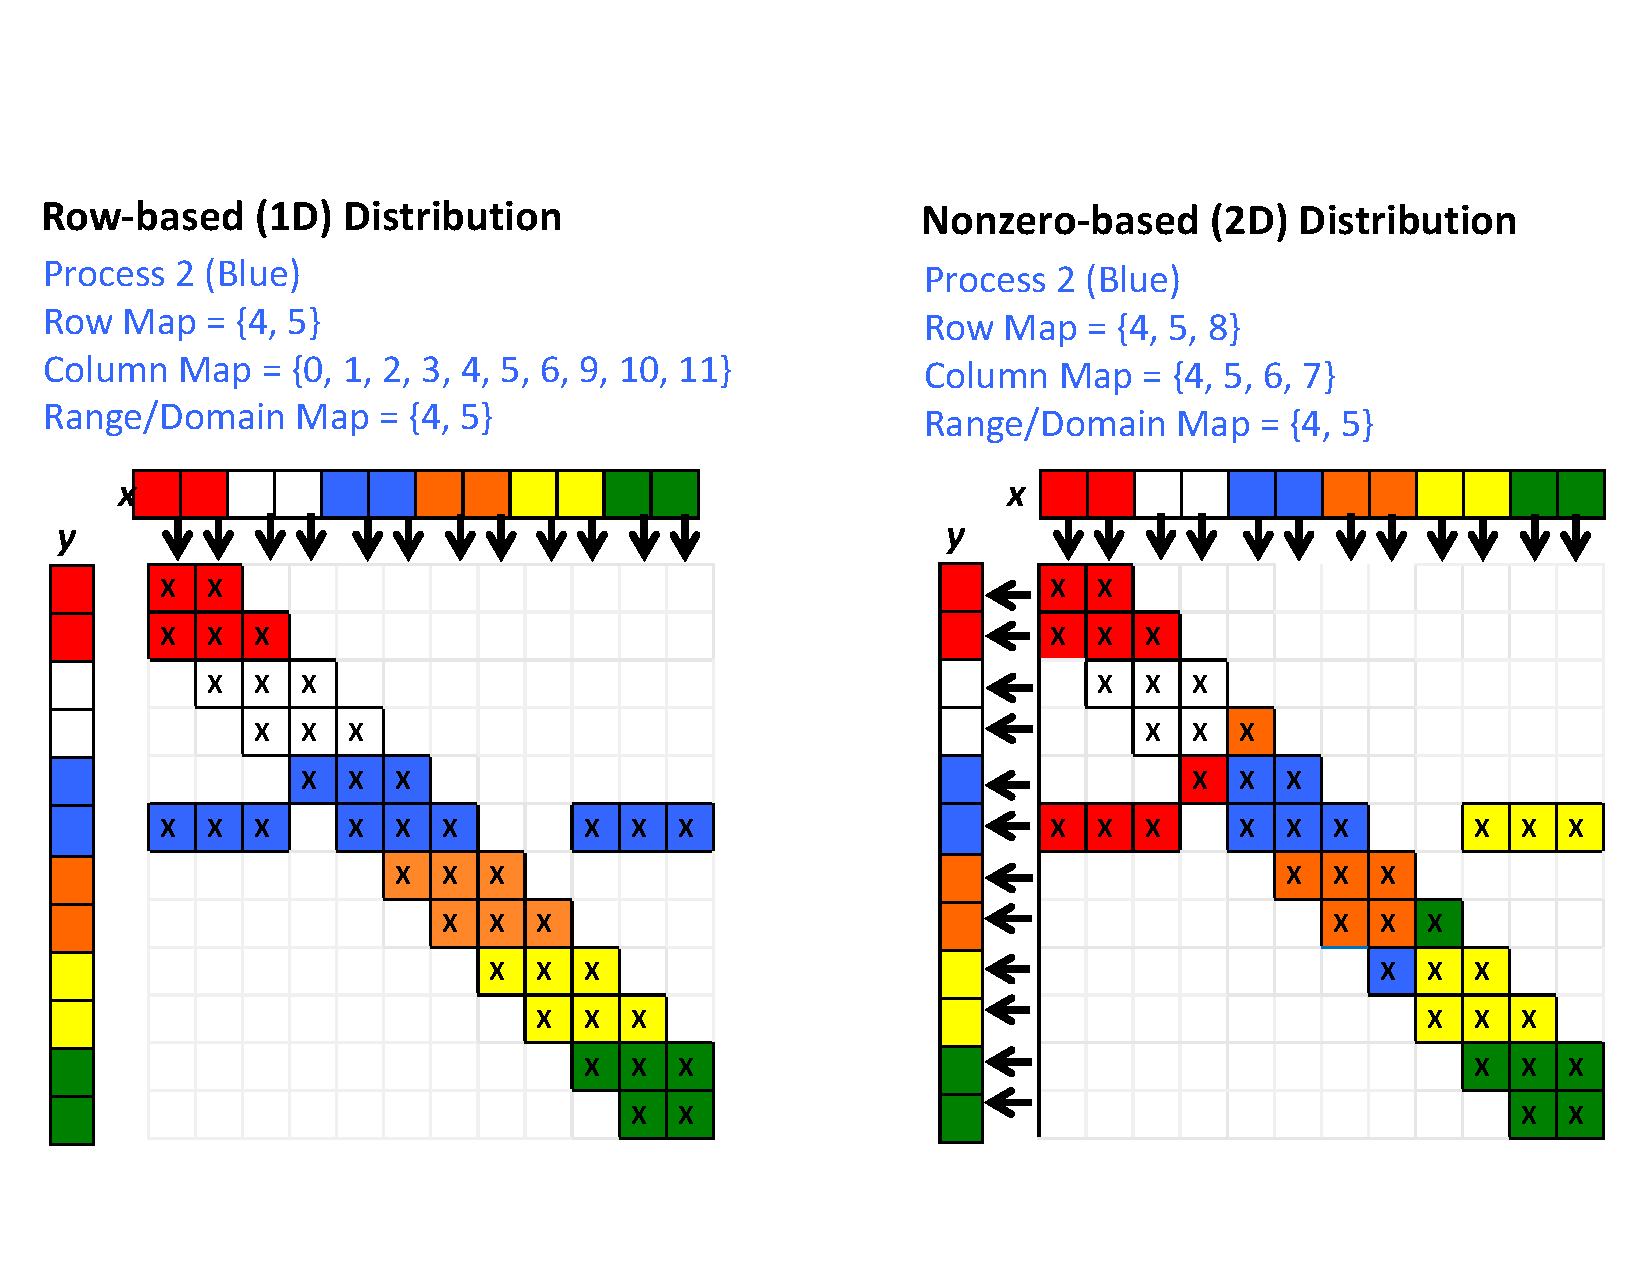
\includegraphics[keepaspectratio=true, width=6in]{figs/trilinosmaps}
   \caption[Examples of a distributed matrix and vectors in Trilinos]{Examples of a distributed matrix and vectors in Trilinos.  The left figure uses a row-based distribution; the right figure uses a nonzero-based distribution.  Colors indicate processor assignment.  The {\tt Map} entries for the blue processor are listed.}
   \label{fig:trilinosmap}
\end{figure}


\section{Tpetra MultiVectors} \label{sec:multivectors}

Tpetra's {\tt MultiVector} class contains $R$ vectors of length $n$, 
distributed to processors according to a Tpetra {\tt Map}.  In Figure
~\ref{fig:trilinosmap}, the input and output vectors $x$ and $y$ are 
{\tt MultiVectors} of length $n=12$ with $R=1$ vector.  They are distributed 
to six processors using ``one-to-one'' maps, so that each entry is uniquely
assigned to a processors.  {\tt MultiVectors} may also have maps that are 
``overlapped'' (not one-to-one) so that multiple processors have copies
of the vectors entries.  Such overlapped maps are used in sparse matrix-vector
multiplication (SpMV), where several processors may contribute to a
single output vector's entry.  (See Chapter~\ref{sec:mttkrp} for details.)
The {\tt MultiVector} class provides operations such as dot products, 
random vector generation, vector normalization, scaling, and vector norms.

\section{Trilinos Communication} \label{sec:import}

Trilinos' Teuchos package provides wrappers around MPI Communicators.
These wrappers allows Trilinos to be built with MPI for parallel execution,
or without it for serial execution.  They wrap the fundamental operations of
MPI (send, receive, reduce, gather), and are used in all of Tpetra's 
distributed objects.

Tpetra provides the class {\tt Import} to establish communication
patterns between pairs of maps.  For example, an {\tt Import} object can be used
to redistribute data from a source MultiVector using one map to a target 
Multivector using a different map.  They can reverse the communication pattern
as well, sending the data from the target object to the source.  Data can be
copied or accumulated into the target object; the latter allows data from
several sources to be added into a single target entry.  An {\tt Import} object
uses point-to-point communication in an underlying Tpetra {\tt Distributor}
class to perform communication.

